\documentclass{article}
\usepackage{geometry}
\usepackage{xcolor}
\usepackage{amsmath}
\usepackage{graphicx}
\usepackage{float}
\usepackage{subcaption}
\usepackage{url}

\geometry{margin=1.5cm}


\begin{document}

\title{Face and Gesture Analysis: Eigenfaces}
\author{Alejandro Fernández Alburquerque, 242349 \\ Andreu Garcies Ramon, 240618}
\date{January 2024}

\maketitle

\textbf{NOTE BEFORE READING:} more images and animated GIFs, as well as the code of the practice, can be seen in the GitHub repository that we have shared with our practice instructor. \url{https://github.com/Alejandro-FA/UPF-Face-and-Gesture-Analysis}

\section{Introduction}
Face detection and recognition have been very important problems in the field of computer vision. They have been subjects of research for many years \cite{adjabi-2020}. Face detection typically employs algorithms to locate and extract facial regions from images or video frames. Popular face detection methods such as Viola-Jones rely on a small number of critical visual features \cite{viola-2004}. Advancements in machine learning, particularly Deep Learning, have significantly improved the accuracy and efficiency of face detection systems through the usage of CNNs such as Multi-task Cascaded Convolutional Networks (MTCNNs) as explained in \cite{xiang-2017}.

In this report, we are going to pay attention to one specific method introduced by Turk and Pentland in the early 1990s \cite{turk-1991}. Although it can be used both for face detection and face recognition, we are not going to apply it for these purposes. We will see how it works on a fundamental theoretical basis. The method works by projecting face images into a feature space that captures the most significant variations of the images. This is done through Principal Component Analysis (PCA), and the method is known as Eigenfaces, as these "eigenfaces" can be thought of as the eigenvectors of the set of faces. This algorithm can be used in very broad domains such as in security systems or in human-computer interaction applications \cite{rodavia-2016, ramadhani-2017}.

\section{Dataset}\label{dataset_section}
In the field of eigenfaces, a suitable dataset is often a key factor for obtaining useful and insightful results. Notably, for PCA to capture relevant features, removing undesired sources of variation from the images (like illumination changes, pose, facial expression, 2D rotations, translation, and background color) is essential. If the dataset does not satisfy these requirements, an additional preprocessing step is often needed, which is not trivial to get right and is often time-consuming.

Given the above requirements, we have decided to develop our project with the Chicago Faces Dataset \cite{debbie-2015}. It contains 597 neutral faces (non-expressive) of people aged 18 to 40 from various races and genders, and it stands out because of its highly standardized photograph conditions. All images are 2444 pixels wide and 1718 pixels high.

Figure \ref{fig:cfd} shows some examples of the images present in the dataset. All subjects are placed onto a plain white background and wear the same grey t-shirt. Other conditions like the illumination, the expression, and the framing are also carefully controlled.

\begin{figure}[H]
    \centering
    \vspace{0in}
    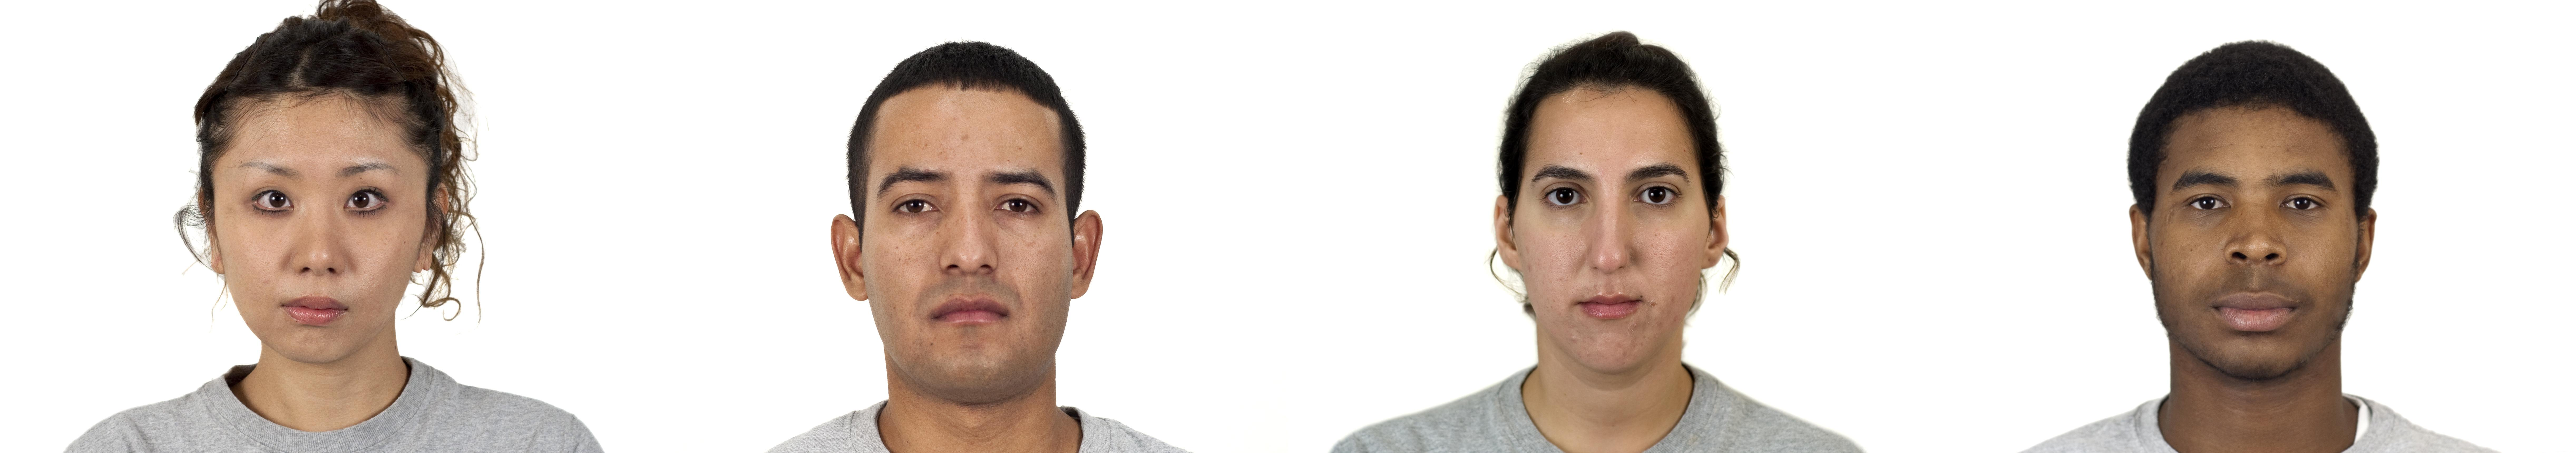
\includegraphics[width=0.8\textwidth]{images/cfd.jpg}
    \caption{Sample of 4 faces included in the Chicago Face Dataset.}
    \label{fig:cfd}
\end{figure}

The last motivation for choosing this database is that landmark templates are also available. The researchers from \cite{singh-2022} have manually placed a set of 189 points to capture the face's shape accurately.


\section{Methodology}

\subsection{Dataset preprocessing}

As explained in \ref{algorithm_section}, the PCA algorithm finds the directions in multidimensional space that capture the most variance. Those directions are related to image features, but if the dataset is not preprocessed adequately, they can correspond to features that do not necessarily discriminate between faces. Fortunately, as mentioned in \ref{dataset_section}, the Chicago Face Dataset already provides images with standardized conditions. For this reason, we have decided not to perform any preprocessing steps regarding illumination, cropping, and rotation. However, to reduce the PCA algorithm's computation time, we have decided to resize the images to a lower resolution (1222 pixels wide by 859 pixels high) and convert them from RGB images to gray-scale images. Figure \ref{fig:preprocessed_images} shows an original image from the dataset along with its preprocessed version.

\begin{figure}[H]
    \centering
    \vspace{0in}
    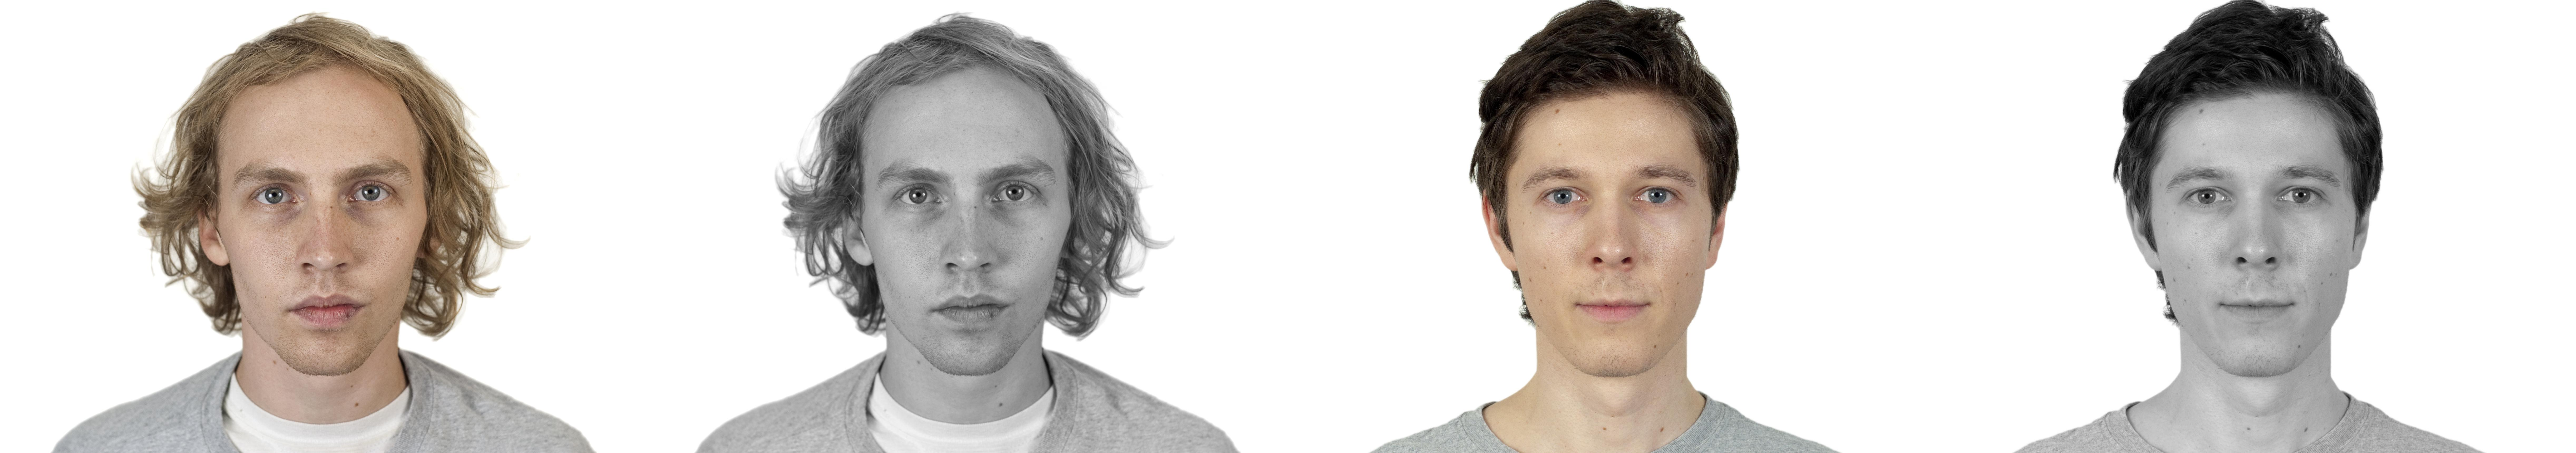
\includegraphics[width=0.8\textwidth]{images/original_vs_preprocessed.jpg}
    \caption{Original images and their corresponding preprocessed images.}
    \label{fig:preprocessed_images}
\end{figure}

Face landmarks usually require less attention than images since they are just a set of points. Since we wanted to be able to plot landmarks on top of the images, we decided to rescale them appropriately to match the new image dimensions. Furthermore, we also decided to remove some of the template points because we did not consider them relevant to our application. Figure \ref{fig:preprocessed_landmarks} shows a comparison between the original landmarks and the preprocessed ones.

\begin{figure}[H]
    \centering
    \vspace{0in}
    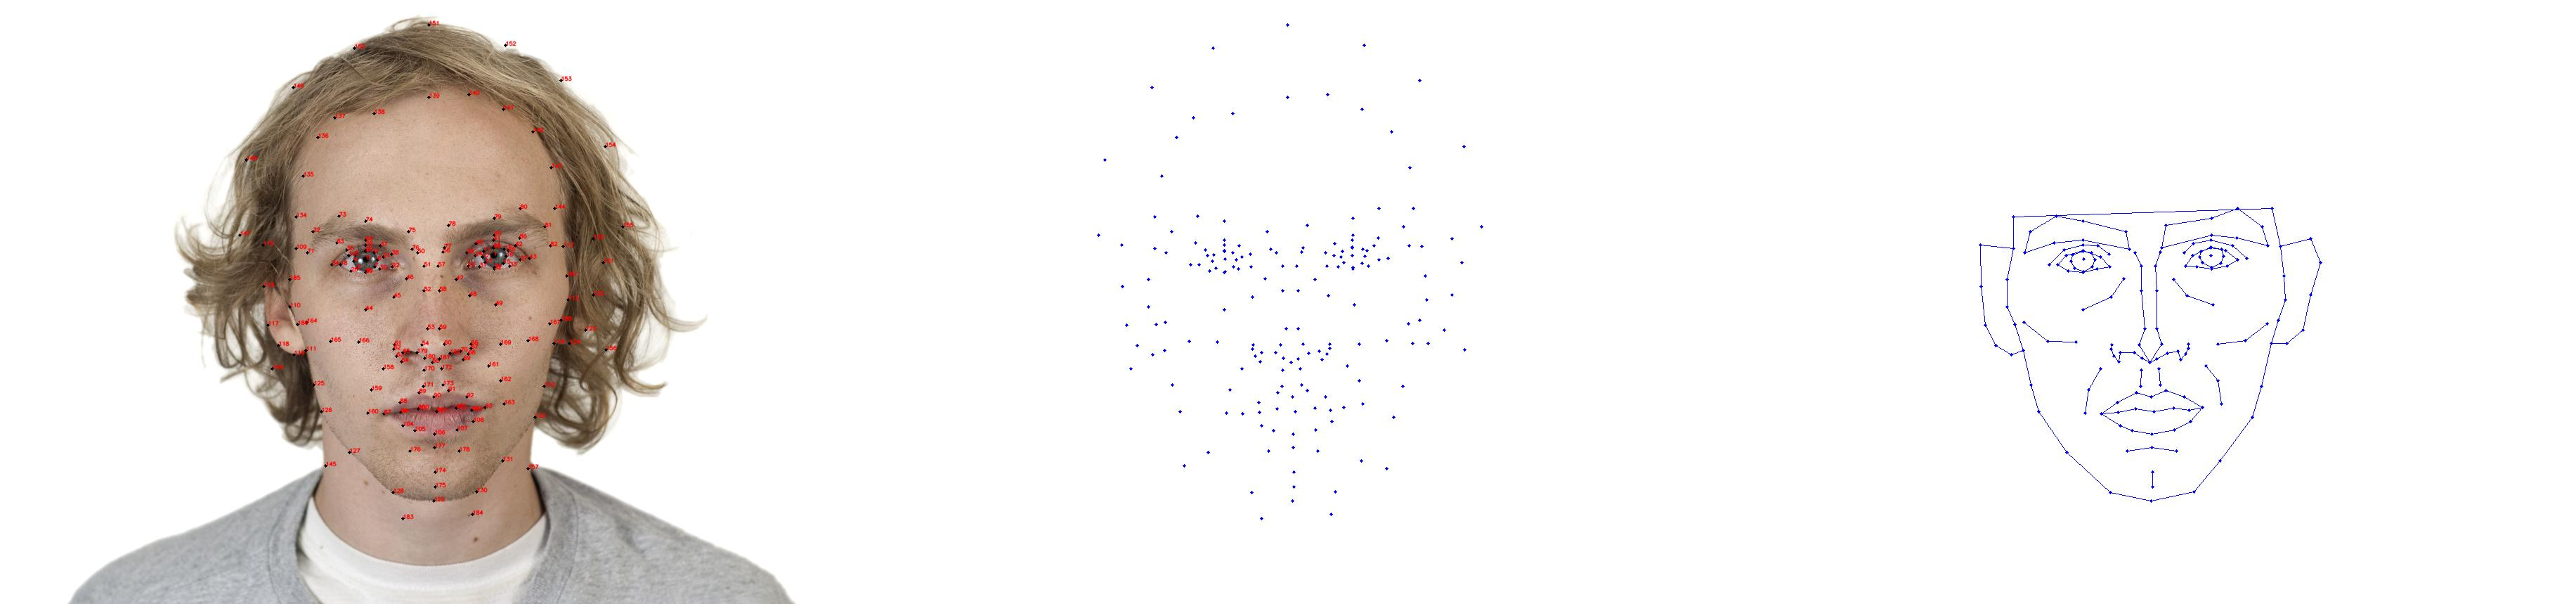
\includegraphics[width=0.8\textwidth]{images/original_vs_preprocessed_landmarks.jpg}
    \caption{Original landmarks and the subset selected for this project.}
    \label{fig:preprocessed_landmarks}
\end{figure}

As a final note, we have not had time to align the landmarks with a Generalized Procrustes Alignment method. The original intention was to do so, but given the limited time and the fact that the landmarks were already quite well aligned, we decided to skip this step.

\subsection{Eigenfaces algorithm}\label{algorithm_section}
The eigenfaces algorithm leverages the power of PCA to represent facial features efficiently in a lower-dimensional space. PCA is a linear dimensionality reduction technique that allows obtaining a lower-dimensional space, the directions of which capture the largest variations of the data in the original space. Throughout this section, we will explain the necessary concepts to understand PCA applied to the task of feature extraction for images and thus generating eigenfaces.

The principal components of a set of data $\mathcal{X}$ are the directions of maximum variance. It can be shown that these principal directions have to be the eigenvectors $\vec{e}_i$ of the covariance matrix $\Sigma$ of the input data. The variance captured by each of each principal direction corresponds to the associated eigenvalue $\lambda_i$ to the eigenvector representing that particular direction. Therefore, the problem of PCA reduces to computing an eigendecomposition of the covariance matrix $\Sigma$, defined as
\begin{equation}\label{cov_matrix}
    \Sigma = \frac{1}{n-1} \sum_{i = 1}^n (x_i - \bar{x})(x_i - \bar{x})^T
\end{equation}
where $n$ refers to the number of samples that the dataset contains. It is key to take into consideration the dimensions of this covariance matrix. If the input data is represented through a $p\times n$ matrix $X$, being $p$ the number of dimensions, then the resulting covariance matrix will be of size $p \times p$. Usually, especially when dealing with image data, $p \gg n$. This means that it is often the case that the covariance matrix $\Sigma$ can not be fitted in memory. With our particular dataset, the covariance matrix as defined in equation \ref{cov_matrix} is of size $1.049.698 \times 1.049.698$, which is enormously big to store in memory (and computationally unfeasible to eigendecompose).

To solve this problem, we can use the pseudo-covariance matrix, which is computed as
\begin{equation}\label{pseudocov_matrix}
    \Sigma^\prime = \frac{1}{n-1} \sum_{i = 1}^n (x_i - \bar{x})^T(x_i - \bar{x})
\end{equation}

The dimensions of this new matrix will be of $n \times n$, which is much more manageable than $\Sigma$. Once we have computed the pseudo-covariance matrix $\Sigma ^\prime$ as stated in equation \ref{pseudocov_matrix}, we should eigendecompose it, obtaining its corresponding eigenvalues ($\lambda_i^\prime$) and eigenvectors ($\vec{e}_i^\prime$).

At this point, we need to remember the original objective of the overall process, which was to obtain $\vec{e}_i$ from $\Sigma$. However, it is very likely that when applying this method to the images from our dataset (the problem does not arise when applying this method to landmarks), we have obtained $\vec{e}_i^\prime$. The eigenvectors from the pseudo-covariance matrix are related to those from the covariance matrix through equation \ref{relation_eigs}
\begin{equation}\label{relation_eigs}
    \vec{e}_i = X \cdot \vec{e}_i^\prime , \space \forall i \in \{1, \dots , n\}
\end{equation}


\subsection{Extracting a meaningful basis}

Having applied the eigenfaces algorithm to our input images, we obtain a basis of $n$ components, each of which accounts for a certain amount of the total variance of the dataset. Even though all the components are required to recover an original exact face given an eigenface (a face in the lower dimensional space spanned by the eigenvectors), not all of them are needed when it comes to obtaining an approximate version of this face. Therefore, a method is required to be able to determine how many of the $n$ components are needed to have a meaningful basis. Several methods exist to decide how many components should be retained. We have chosen to perform significance tests using bootstrap.

With this goal, let us define $p$ tests, where $p$ is the number of dimensions of the data. For each of these $p$ tests, we define a null hypothesis indicating that \textit{the relative variance explained by component p of the PCA basis of the original data is the same as that of the relative variance explained by component p of the PCA basis of uncorrelated data}. It is important to note that here, we assume that the PCA basis is sorted in descending order according to the eigenvalues. Mathematically, the null hypothesis is defined as $H_{0,p}: \lambda_p = \hat{\lambda}_p$, where $\hat{\lambda}_p$ corresponds to the eigenvalue of uncorrelated data. The alternative hypothesis is $H_{A,p}: \lambda_p > \hat{\lambda}_p$.

To test all the hypotheses, we have used $B = 100$ permutation tests. For each of these tests, a p-value is computed. This p-value represents the probability of observing a result as extreme as (or more) than the ones observed, assuming that $H_0$ is true. At significance level $\alpha$, $H_0$ cannot be rejected as long as $\text{p-value} < \alpha$ holds. Finally, once all tests have been performed, we consider that there are $k$ significant components if we have been able to reject the null hypothesis with $\alpha = 0.05$ of $k$ tests. The results of these tests for images and landmarks can be seen in Figure \ref{fig:scree_plots}.

For the images of the faces, our results indicate that the meaningful basis with $\alpha = 0.05$ is that containing 33 components. This means that, on average, 95\% of the time, the variance explained by each of the first 33 principal components (81.6\%) of our basis will be higher than if we were using uncorrelated data. A similar reasoning applies to landmarks.



\begin{figure}[H]
    \centering

    \begin{subfigure}{0.7\textwidth}
        \centering
        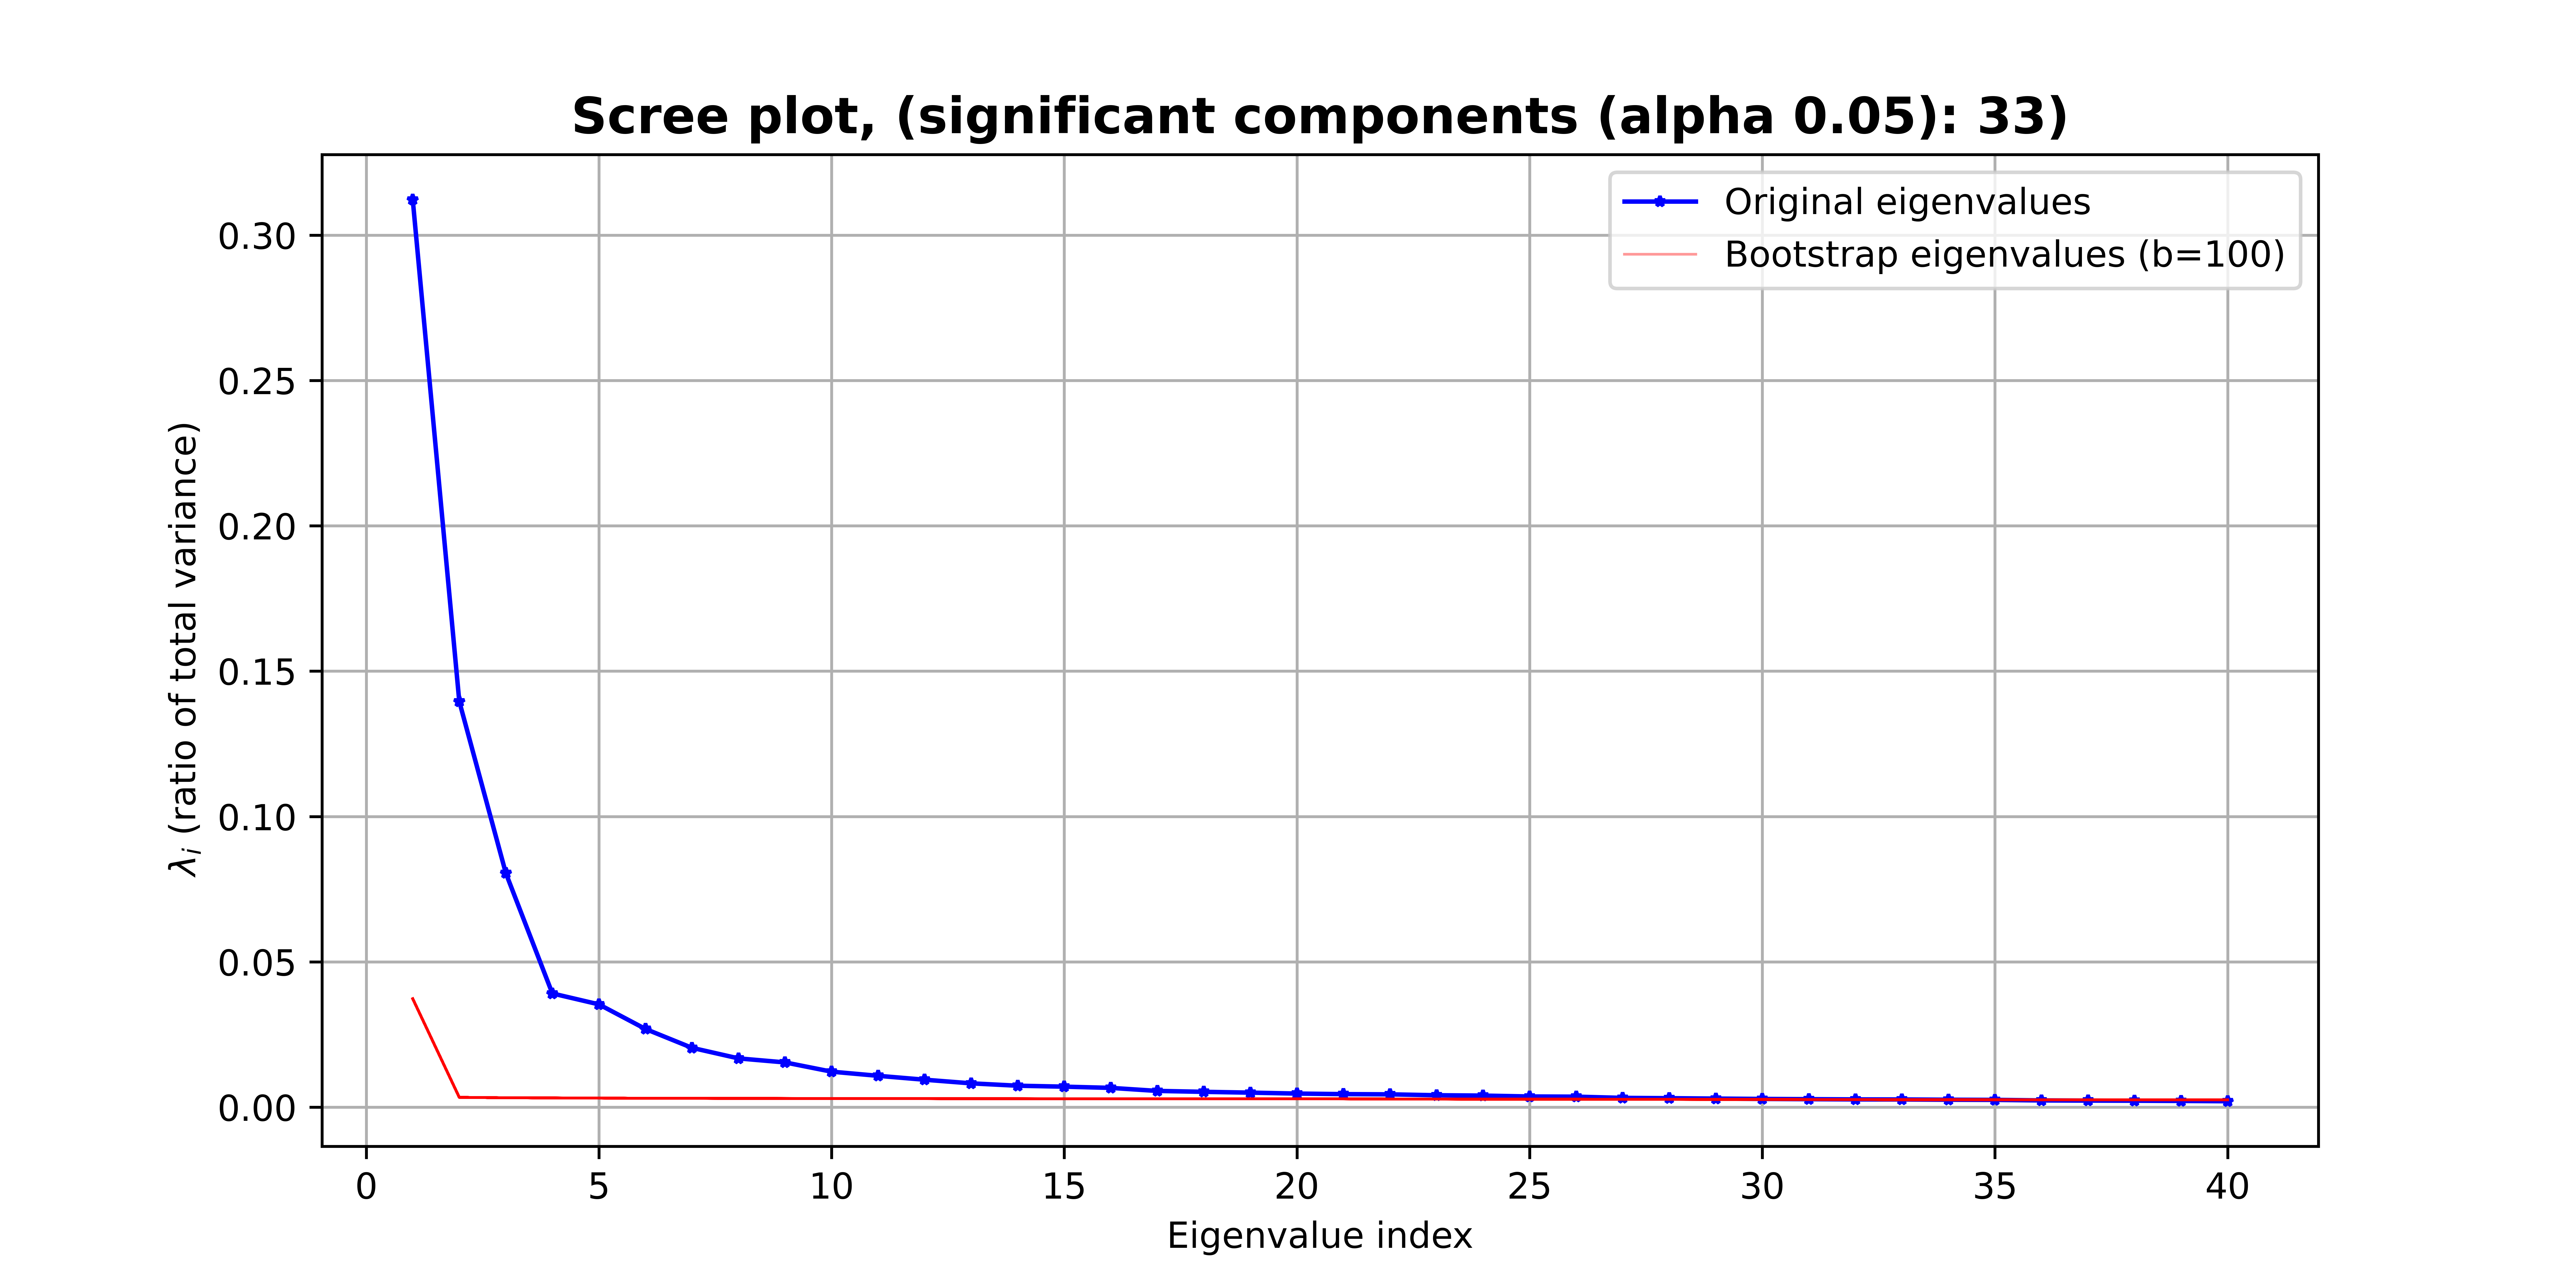
\includegraphics[width=\linewidth]{images/images_scree_plot.png}
        \caption{Hypothesis testing for the images.}
        \label{fig:scree_plot_images}
    \end{subfigure}
    % \hfill
    \begin{subfigure}{0.7\textwidth}
        \centering
        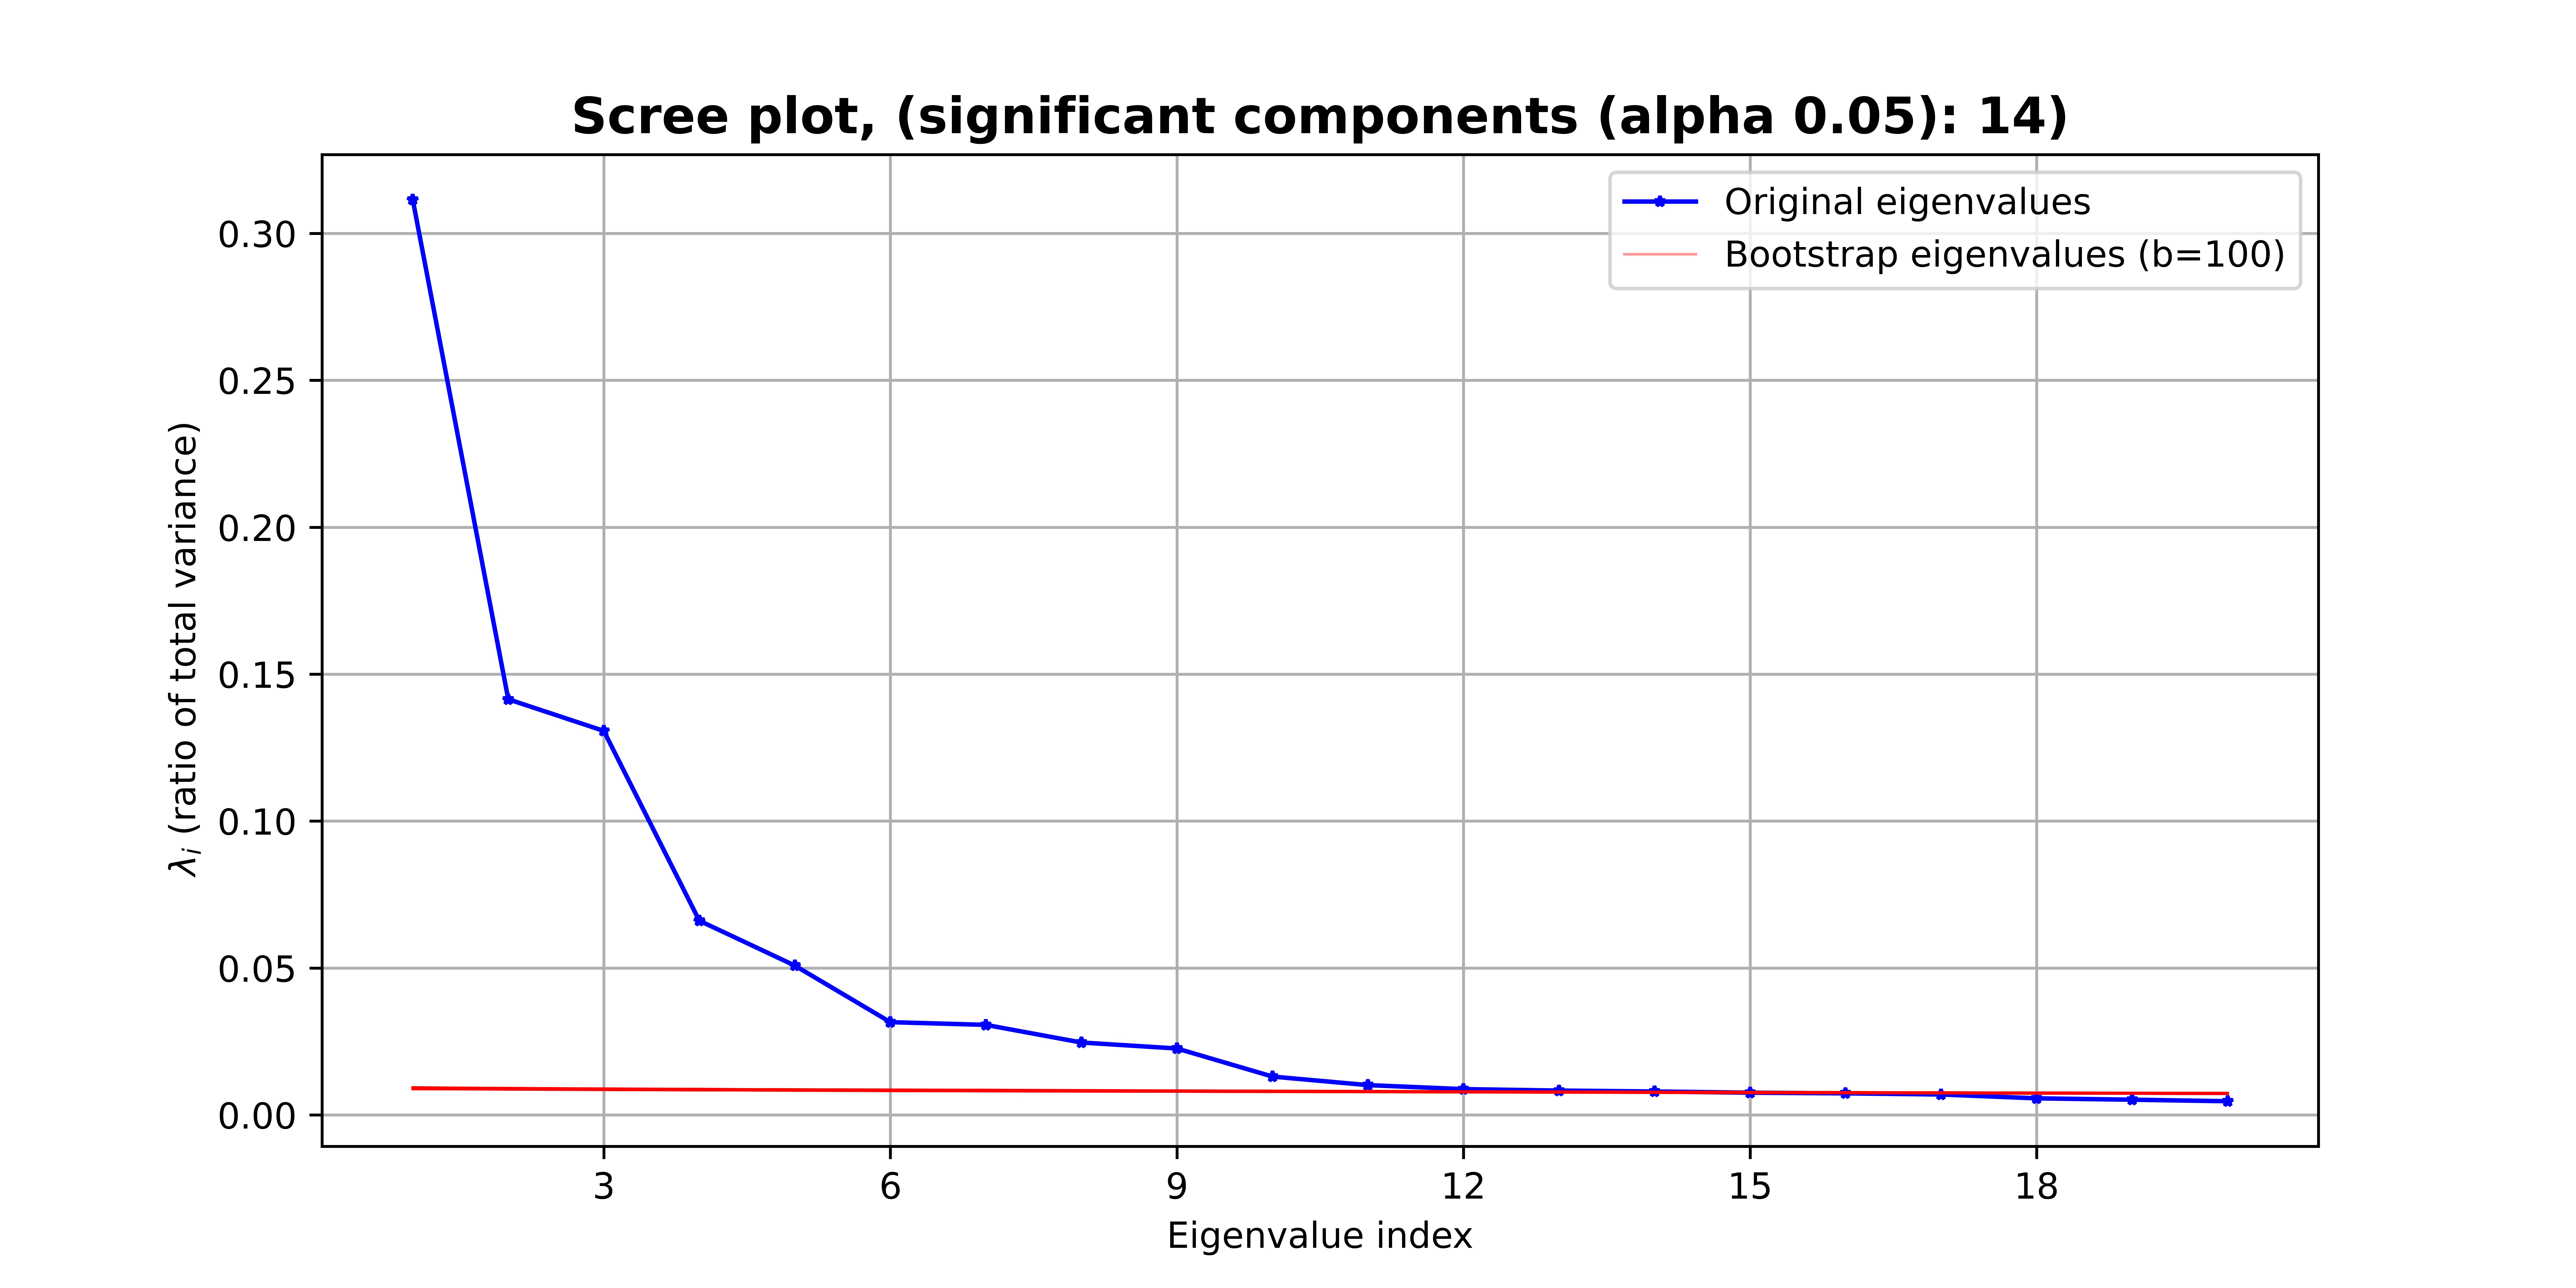
\includegraphics[width=\linewidth]{images/landmarks_scree_plot.png}
        \caption{Hypothesis testing for the landmarks.}
        \label{fig:scree_plot_landmarks}
    \end{subfigure}

    \caption{Comparison of scree plots for images and landmarks.}
    \label{fig:scree_plots}
\end{figure}



\section{Results}

\subsection{Images reconstruction in a lower-dimensional basis}

This part of the report aims to visually see how we can use the basis we have obtained to generate meaningful lower-dimensional representations of the faces. Since the first components of the eigenfaces basis capture the largest proportion of total variance, it is interesting to interpret the results as a form of image compression. For example, if instead of storing the full $1.049.698$ of pixels of the image, we only save the first 33 components, we would only need to store $19.569$ values. Therefore, we would go from an 800 KB image to a file of only 15 KB. In a more realistic scenario, we could increase the number of stored PCA components to 300, which would still imply a significant compression with an output file at around 136 KB. Figure \ref{fig:reconstructed_images} shows two examples of the effect of "compressing" the image to PCA space and then recovering it back to a 1222 x 859 image.

\begin{figure}[H]
    \centering

    \begin{subfigure}{0.7\textwidth}
        \centering
        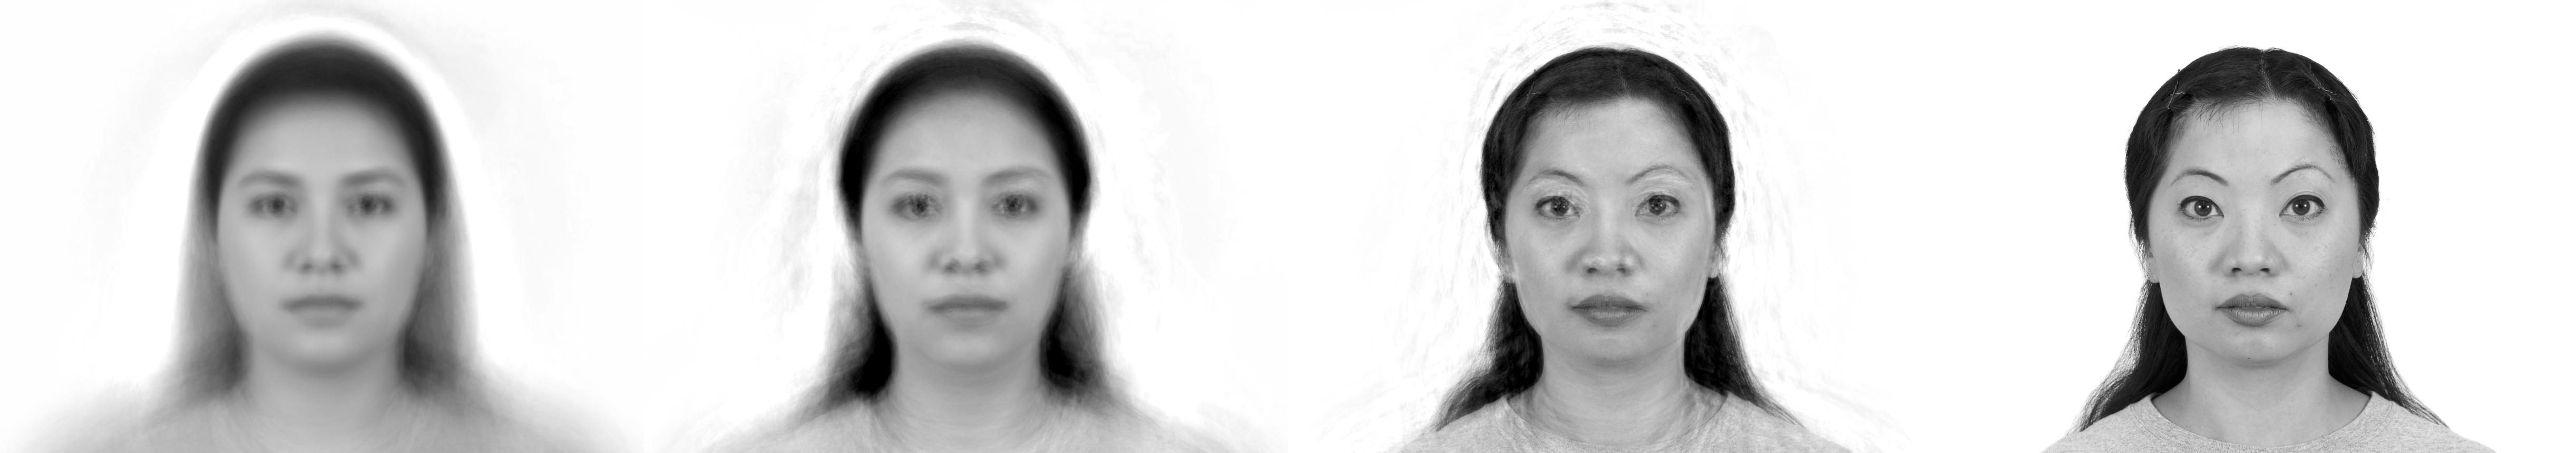
\includegraphics[width=\linewidth]{images/reconstructed_1.jpg}
        % \caption{Hypothesis testing for the images.}
        \label{fig:reconstructed_1}
    \end{subfigure}
    % \hfill
    \begin{subfigure}{0.7\textwidth}
        \centering
        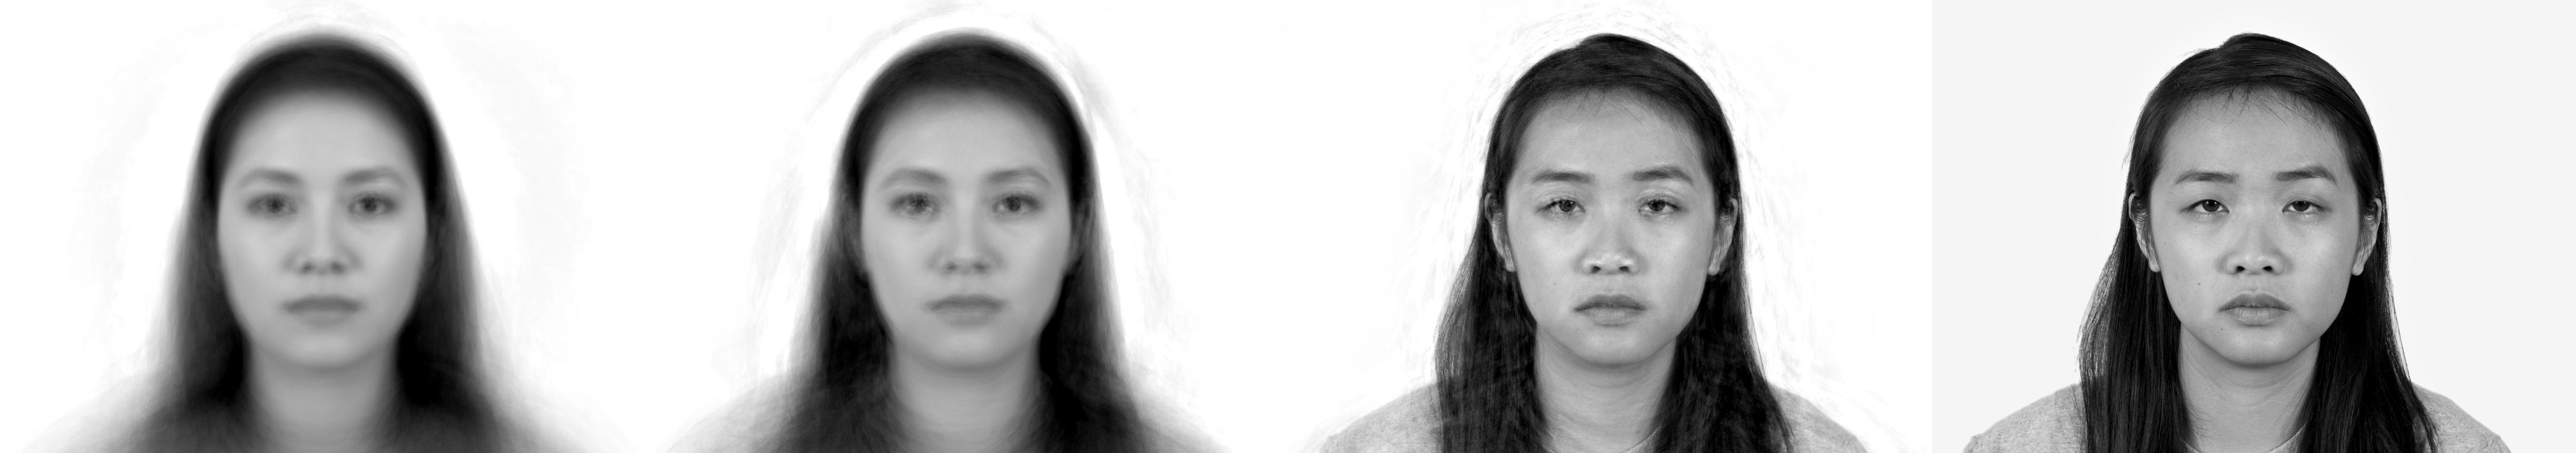
\includegraphics[width=\linewidth]{images/reconstructed_2.jpg}
        % \caption{Hypothesis testing for the landmarks.}
        \label{fig:reconstrued_2}
    \end{subfigure}

    \caption{Two examples of image reconstruction with 10, 33, 300 and 596 principal components, respectively.}
    \label{fig:reconstructed_images}
\end{figure}

It is important to note that obtaining a perfect reconstruction for this application is impossible because our data has more dimensions than samples. This problem is absent when doing a similar analysis for the landmarks because, in that case, the number of samples is larger than the number of dimensions. Furthermore, the reconstruction can be hampered by numerical errors since we need to round floating-point pixel values to integers before plotting the image. A combination of these errors might be used to explain the difference in background color in \ref{fig:reconstructed_images}. In the reconstruction with 596 components of the second face, the background color is not white (something that does not happen in the original image).

\subsection{Modes of variation}

The eigenfaces serve as vectors representing the directions of a new coordinate system centered around the mean image $\bar{x}$. Consequently, when traversing along each principal component, deviations from $\bar{x}$ represent faces that distinguish from it on the specific feature captured by that principal component. For each of the meaningful components, we have generated new facial images as $x_\text{new} = \bar{x} + \vec{e}_i \cdot \text{offset}$ with $\text{offset} \in \left[-3 \cdot \sqrt{\lambda_i}, 3 \cdot \sqrt{\lambda_i}\right]$. Some of the results are presented in figures \ref{fig:images_modes_of_variation} and \ref{fig:landmarks_modes_of_variation}.

For the images, it looks like the first component mainly captures the gender of the face appearing in the image. It generates from female-looking faces with longer hair to male-looking faces with less hair. It is more difficult to identify a clear feature for the second component. It could be said that it captures subtle differences in facial features that distinguish between white and black people. The third component clearly captures the skin color. It generates neutral-looking faces with a wide range of skin color.

\begin{figure}[H]
    \centering

    \begin{subfigure}[b]{0.8\textwidth}
        \centering
        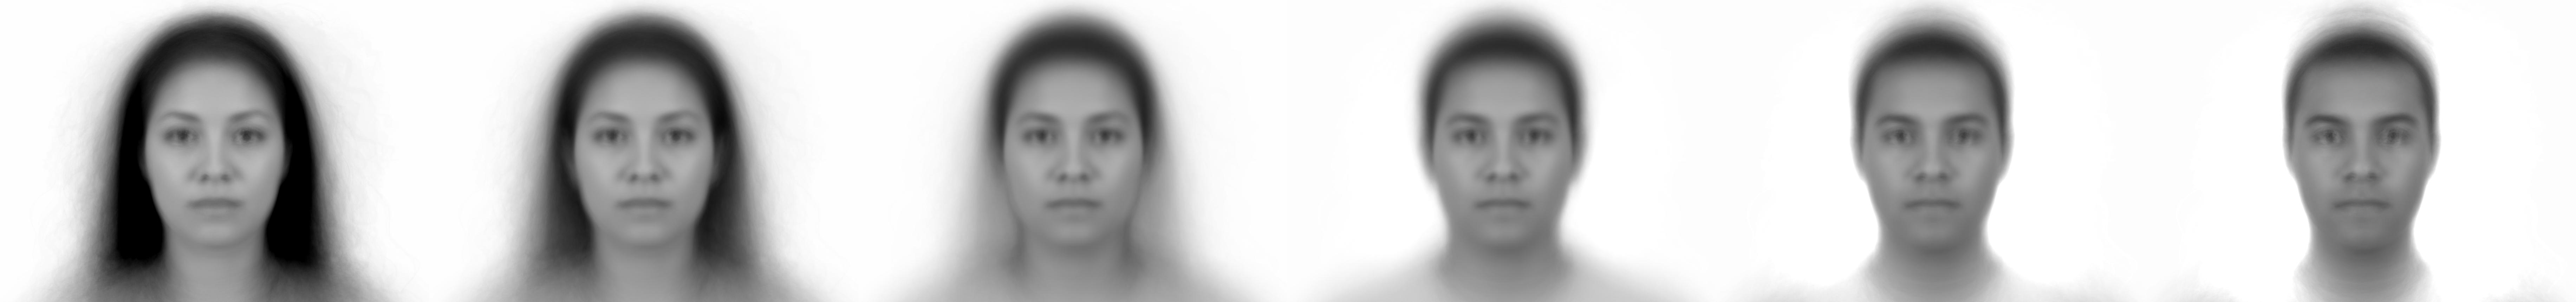
\includegraphics[width=\linewidth]{images/mv_image_eigenvector_0.jpg}
        \caption{1st eigenvector.}
        \label{fig:preprocessed_landmarks}
    \end{subfigure}

    % \vspace{0.2in} % Adjust the vertical space between subfigures

    \begin{subfigure}[b]{0.8\textwidth}
        \centering
        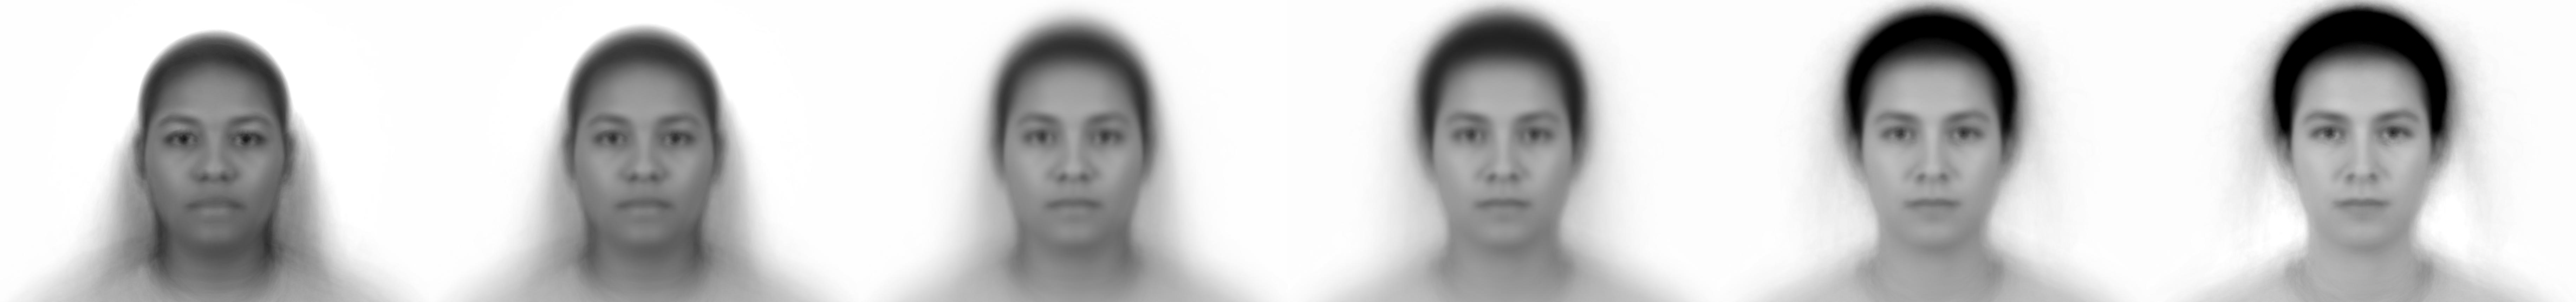
\includegraphics[width=\linewidth]{images/mv_image_eigenvector_1.jpg}
        \caption{2nd eigenvector.}
        \label{fig:second_repetition}
    \end{subfigure}

    % \vspace{0.2in} % Adjust the vertical space between subfigures

    \begin{subfigure}[b]{0.8\textwidth}
        \centering
        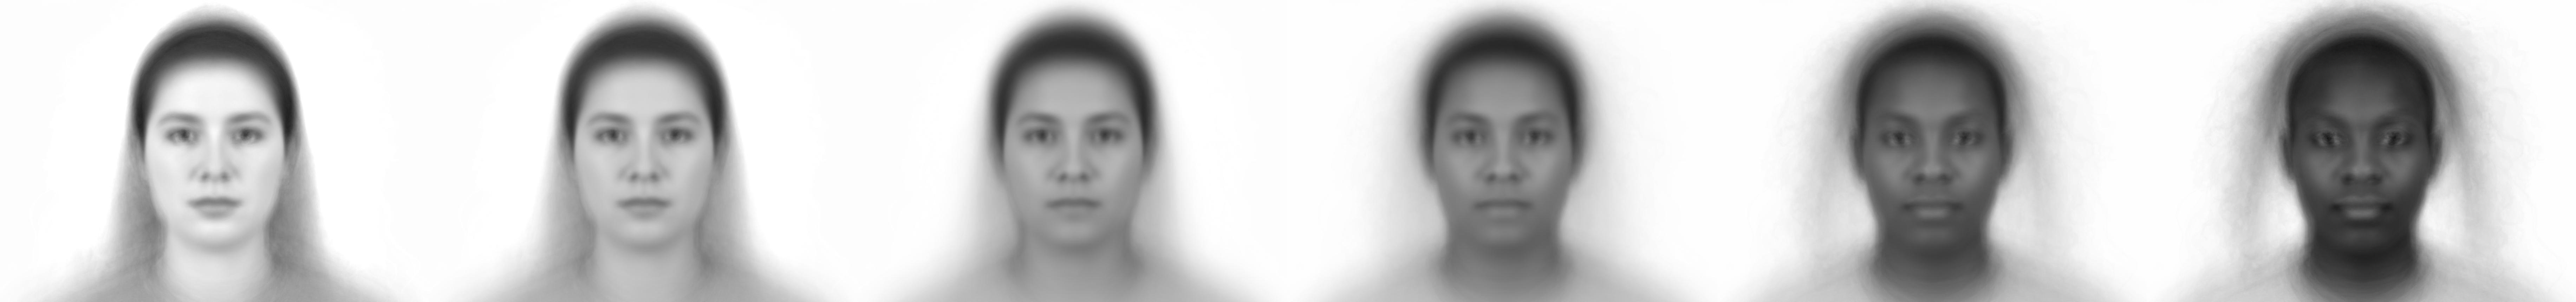
\includegraphics[width=\linewidth]{images/mv_image_eigenvector_2.jpg}
        \caption{3rd eigenvector.}
        \label{fig:third_repetition}
    \end{subfigure}

    \caption{Images modes of variation}
    \label{fig:images_modes_of_variation}
\end{figure}

Identifying the features captured by the eigenfaces corresponding to the landmarks is much more difficult. From the three eigenvectors shown in Figure \ref{fig:landmarks_modes_of_variation}, the most notable feature is the change in face longitude captured by the second eigenvector. Other variations seem to capture 3D rotations.

\begin{figure}[H]
    \centering

    \begin{subfigure}[b]{0.8\textwidth}
        \centering
        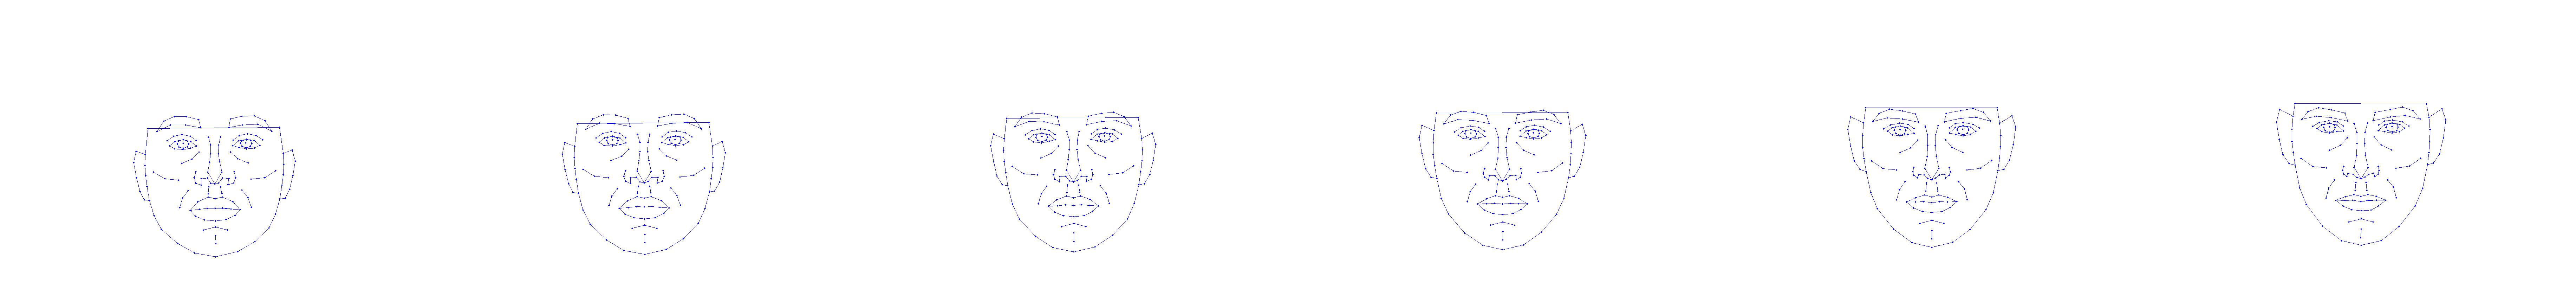
\includegraphics[width=\linewidth]{images/mv_landmarks_eigenvector_0.jpg}
        \caption{1st eigenvector.}
        \label{fig:preprocessed_landmarks}
    \end{subfigure}

    % \vspace{0.2in} % Adjust the vertical space between subfigures

    \begin{subfigure}[b]{0.8\textwidth}
        \centering
        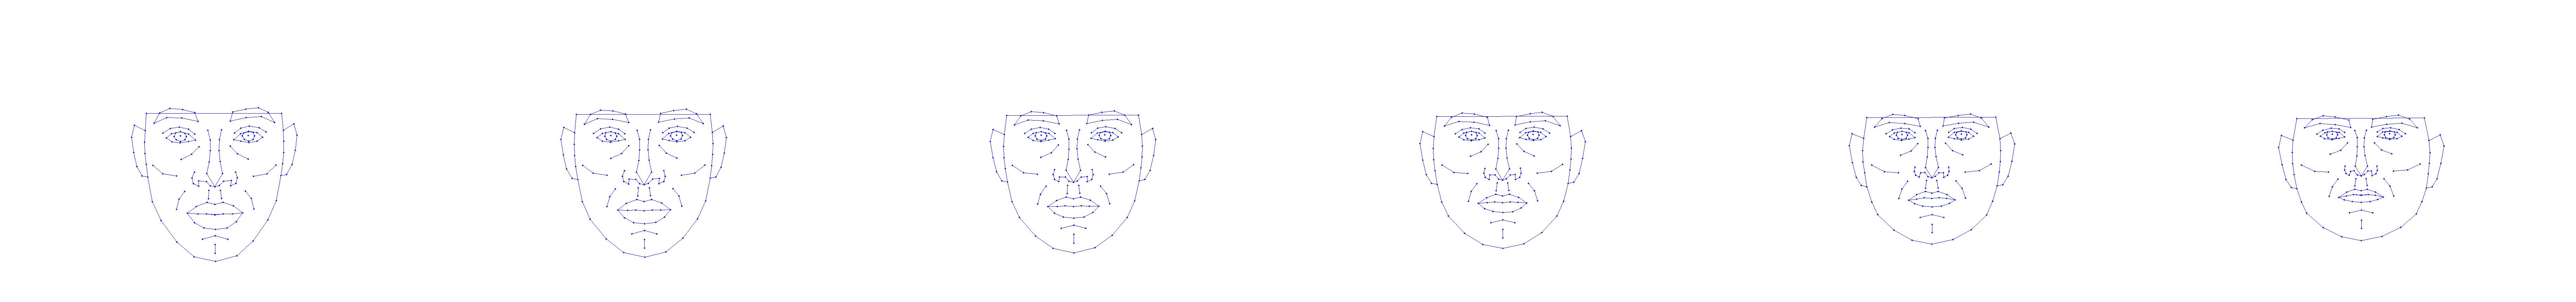
\includegraphics[width=\linewidth]{images/mv_landmarks_eigenvector_1.jpg}
        \caption{2nd eigenvector.}
        \label{fig:second_repetition}
    \end{subfigure}

    % \vspace{0.2in} % Adjust the vertical space between subfigures

    \begin{subfigure}[b]{0.8\textwidth}
        \centering
        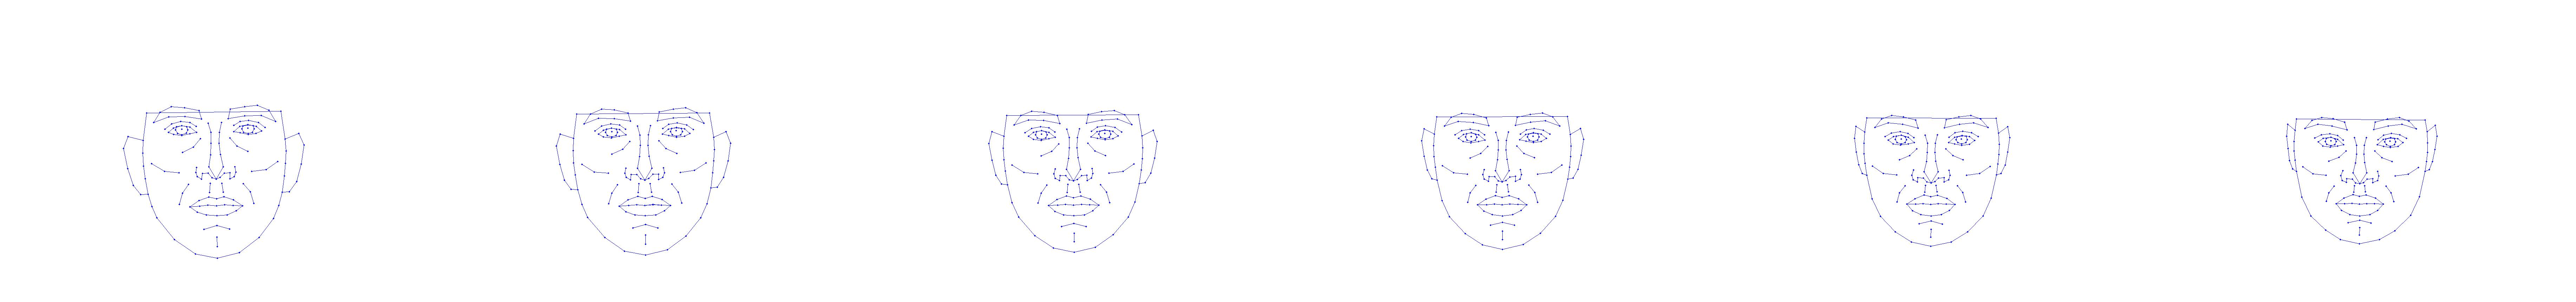
\includegraphics[width=\linewidth]{images/mv_landmarks_eigenvector_2.jpg}
        \caption{3rd eigenvector.}
        \label{fig:third_repetition}
    \end{subfigure}

    \caption{Landmarks modes of variation}
    \label{fig:landmarks_modes_of_variation}
\end{figure}

\newpage
\bibliographystyle{apalike}
\bibliography{refs}

\end{document}
